
%% bare_conf.tex
%% V1.3
%% 2007/01/11
%% by Michael Shell
%% See:
%% http://www.michaelshell.org/
%% for current contact information.
%%
%% This is a skeleton file demonstrating the use of IEEEtran.cls
%% (requires IEEEtran.cls version 1.7 or later) with an IEEE conference paper.
%%
%% Support sites:
%% http://www.michaelshell.org/tex/ieeetran/
%% http://www.ctan.org/tex-archive/macros/latex/contrib/IEEEtran/
%% and
%% http://www.ieee.org/

%%*************************************************************************
%% Legal Notice:
%% This code is offered as-is without any warranty either expressed or
%% implied; without even the implied warranty of MERCHANTABILITY or
%% FITNESS FOR A PARTICULAR PURPOSE!
%% User assumes all risk.
%% In no event shall IEEE or any contributor to this code be liable for
%% any damages or losses, including, but not limited to, incidental,
%% consequential, or any other damages, resulting from the use or misuse
%% of any information contained here.
%%
%% All comments are the opinions of their respective authors and are not
%% necessarily endorsed by the IEEE.
%%
%% This work is distributed under the LaTeX Project Public License (LPPL)
%% ( http://www.latex-project.org/ ) version 1.3, and may be freely used,
%% distributed and modified. A copy of the LPPL, version 1.3, is included
%% in the base LaTeX documentation of all distributions of LaTeX released
%% 2003/12/01 or later.
%% Retain all contribution notices and credits.
%% ** Modified files should be clearly indicated as such, including  **
%% ** renaming them and changing author support contact information. **
%%
%% File list of work: IEEEtran.cls, IEEEtran_HOWTO.pdf, bare_adv.tex,
%%                    bare_conf.tex, bare_jrnl.tex, bare_jrnl_compsoc.tex
%%*************************************************************************

% *** Authors should verify (and, if needed, correct) their LaTeX system  ***
% *** with the testflow diagnostic prior to trusting their LaTeX platform ***
% *** with production work. IEEE's font choices can trigger bugs that do  ***
% *** not appear when using other class files.                            ***
% The testflow support page is at:
% http://www.michaelshell.org/tex/testflow/



% Note that the a4paper option is mainly intended so that authors in
% countries using A4 can easily print to A4 and see how their papers will
% look in print - the typesetting of the document will not typically be
% affected with changes in paper size (but the bottom and side margins will).
% Use the testflow package mentioned above to verify correct handling of
% both paper sizes by the user's LaTeX system.
%
% Also note that the "draftcls" or "draftclsnofoot", not "draft", option
% should be used if it is desired that the figures are to be displayed in
% draft mode.
%
\documentclass[conference]{IEEEtran}
% Add the compsoc option for Computer Society conferences.
%
% If IEEEtran.cls has not been installed into the LaTeX system files,
% manually specify the path to it like:
% \documentclass[conference]{../sty/IEEEtran}


\IEEEoverridecommandlockouts %To add sponsors and index terms


% Some very useful LaTeX packages include:
% (uncomment the ones you want to load)


% *** MISC UTILITY PACKAGES ***
%
%\usepackage{ifpdf}
% Heiko Oberdiek's ifpdf.sty is very useful if you need conditional
% compilation based on whether the output is pdf or dvi.
% usage:
% \ifpdf
%   % pdf code
% \else
%   % dvi code
% \fi
% The latest version of ifpdf.sty can be obtained from:
% http://www.ctan.org/tex-archive/macros/latex/contrib/oberdiek/
% Also, note that IEEEtran.cls V1.7 and later provides a builtin
% \ifCLASSINFOpdf conditional that works the same way.
% When switching from latex to pdflatex and vice-versa, the compiler may
% have to be run twice to clear warning/error messages.




\usepackage{comment}

% *** CITATION PACKAGES ***
%
\usepackage{cite}
% cite.sty was written by Donald Arseneau
% V1.6 and later of IEEEtran pre-defines the format of the cite.sty package
% \cite{} output to follow that of IEEE. Loading the cite package will
% result in citation numbers being automatically sorted and properly
% "compressed/ranged". e.g., [1], [9], [2], [7], [5], [6] without using
% cite.sty will become [1], [2], [5]--[7], [9] using cite.sty. cite.sty's
% \cite will automatically add leading space, if needed. Use cite.sty's
% noadjust option (cite.sty V3.8 and later) if you want to turn this off.
% cite.sty is already installed on most LaTeX systems. Be sure and use
% version 4.0 (2003-05-27) and later if using hyperref.sty. cite.sty does
% not currently provide for hyperlinked citations.
% The latest version can be obtained at:
% http://www.ctan.org/tex-archive/macros/latex/contrib/cite/
% The documentation is contained in the cite.sty file itself.






% *** GRAPHICS RELATED PACKAGES ***
%
\ifCLASSINFOpdf
   \usepackage[pdftex]{graphicx}
  % declare the path(s) where your graphic files are
   \graphicspath{{./Images/}}
  % and their extensions so you won't have to specify these with
  % every instance of \includegraphics
   \DeclareGraphicsExtensions{.pdf,.jpeg,.png}
\else
  % or other class option (dvipsone, dvipdf, if not using dvips). graphicx
  % will default to the driver specified in the system graphics.cfg if no
  % driver is specified.
  % \usepackage[dvips]{graphicx}
  % declare the path(s) where your graphic files are
  % \graphicspath{{../eps/}}
  % and their extensions so you won't have to specify these with
  % every instance of \includegraphics
  % \DeclareGraphicsExtensions{.eps}
\fi
% graphicx was written by David Carlisle and Sebastian Rahtz. It is
% required if you want graphics, photos, etc. graphicx.sty is already
% installed on most LaTeX systems. The latest version and documentation can
% be obtained at:
% http://www.ctan.org/tex-archive/macros/latex/required/graphics/
% Another good source of documentation is "Using Imported Graphics in
% LaTeX2e" by Keith Reckdahl which can be found as epslatex.ps or
% epslatex.pdf at: http://www.ctan.org/tex-archive/info/
%
% latex, and pdflatex in dvi mode, support graphics in encapsulated
% postscript (.eps) format. pdflatex in pdf mode supports graphics
% in .pdf, .jpeg, .png and .mps (metapost) formats. Users should ensure
% that all non-photo figures use a vector format (.eps, .pdf, .mps) and
% not a bitmapped formats (.jpeg, .png). IEEE frowns on bitmapped formats
% which can result in "jaggedy"/blurry rendering of lines and letters as
% well as large increases in file sizes.
%
% You can find documentation about the pdfTeX application at:
% http://www.tug.org/applications/pdftex





% *** MATH PACKAGES ***
%
\usepackage[cmex10]{amsmath}
% A popular package from the American Mathematical Society that provides
% many useful and powerful commands for dealing with mathematics. If using
% it, be sure to load this package with the cmex10 option to ensure that
% only type 1 fonts will utilized at all point sizes. Without this option,
% it is possible that some math symbols, particularly those within
% footnotes, will be rendered in bitmap form which will result in a
% document that can not be IEEE Xplore compliant!
%
% Also, note that the amsmath package sets \interdisplaylinepenalty to 10000
% thus preventing page breaks from occurring within multiline equations. Use:
%\interdisplaylinepenalty=2500
% after loading amsmath to restore such page breaks as IEEEtran.cls normally
% does. amsmath.sty is already installed on most LaTeX systems. The latest
% version and documentation can be obtained at:
% http://www.ctan.org/tex-archive/macros/latex/required/amslatex/math/





% *** SPECIALIZED LIST PACKAGES ***
%
%\usepackage{algorithmic}
% algorithmic.sty was written by Peter Williams and Rogerio Brito.
% This package provides an algorithmic environment fo describing algorithms.
% You can use the algorithmic environment in-text or within a figure
% environment to provide for a floating algorithm. Do NOT use the algorithm
% floating environment provided by algorithm.sty (by the same authors) or
% algorithm2e.sty (by Christophe Fiorio) as IEEE does not use dedicated
% algorithm float types and packages that provide these will not provide
% correct IEEE style captions. The latest version and documentation of
% algorithmic.sty can be obtained at:
% http://www.ctan.org/tex-archive/macros/latex/contrib/algorithms/
% There is also a support site at:
% http://algorithms.berlios.de/index.html
% Also of interest may be the (relatively newer and more customizable)
% algorithmicx.sty package by Szasz Janos:
% http://www.ctan.org/tex-archive/macros/latex/contrib/algorithmicx/




% *** ALIGNMENT PACKAGES ***
%
%\usepackage{array}
% Frank Mittelbach's and David Carlisle's array.sty patches and improves
% the standard LaTeX2e array and tabular environments to provide better
% appearance and additional user controls. As the default LaTeX2e table
% generation code is lacking to the point of almost being broken with
% respect to the quality of the end results, all users are strongly
% advised to use an enhanced (at the very least that provided by array.sty)
% set of table tools. array.sty is already installed on most systems. The
% latest version and documentation can be obtained at:
% http://www.ctan.org/tex-archive/macros/latex/required/tools/


%\usepackage{mdwmath}
%\usepackage{mdwtab}
% Also highly recommended is Mark Wooding's extremely powerful MDW tools,
% especially mdwmath.sty and mdwtab.sty which are used to format equations
% and tables, respectively. The MDWtools set is already installed on most
% LaTeX systems. The lastest version and documentation is available at:
% http://www.ctan.org/tex-archive/macros/latex/contrib/mdwtools/


% IEEEtran contains the IEEEeqnarray family of commands that can be used to
% generate multiline equations as well as matrices, tables, etc., of high
% quality.


%\usepackage{eqparbox}
% Also of notable interest is Scott Pakin's eqparbox package for creating
% (automatically sized) equal width boxes - aka "natural width parboxes".
% Available at:
% http://www.ctan.org/tex-archive/macros/latex/contrib/eqparbox/





% *** SUBFIGURE PACKAGES ***
%\usepackage[tight,footnotesize]{subfigure}
% subfigure.sty was written by Steven Douglas Cochran. This package makes it
% easy to put subfigures in your figures. e.g., "Figure 1a and 1b". For IEEE
% work, it is a good idea to load it with the tight package option to reduce
% the amount of white space around the subfigures. subfigure.sty is already
% installed on most LaTeX systems. The latest version and documentation can
% be obtained at:
% http://www.ctan.org/tex-archive/obsolete/macros/latex/contrib/subfigure/
% subfigure.sty has been superceeded by subfig.sty.



%\usepackage[caption=false]{caption}
%\usepackage[font=footnotesize]{subfig}
% subfig.sty, also written by Steven Douglas Cochran, is the modern
% replacement for subfigure.sty. However, subfig.sty requires and
% automatically loads Axel Sommerfeldt's caption.sty which will override
% IEEEtran.cls handling of captions and this will result in nonIEEE style
% figure/table captions. To prevent this problem, be sure and preload
% caption.sty with its "caption=false" package option. This is will preserve
% IEEEtran.cls handing of captions. Version 1.3 (2005/06/28) and later
% (recommended due to many improvements over 1.2) of subfig.sty supports
% the caption=false option directly:
%\usepackage[caption=false,font=footnotesize]{subfig}
%
% The latest version and documentation can be obtained at:
% http://www.ctan.org/tex-archive/macros/latex/contrib/subfig/
% The latest version and documentation of caption.sty can be obtained at:
% http://www.ctan.org/tex-archive/macros/latex/contrib/caption/




% *** FLOAT PACKAGES ***
%
%\usepackage{fixltx2e}
% fixltx2e, the successor to the earlier fix2col.sty, was written by
% Frank Mittelbach and David Carlisle. This package corrects a few problems
% in the LaTeX2e kernel, the most notable of which is that in current
% LaTeX2e releases, the ordering of single and double column floats is not
% guaranteed to be preserved. Thus, an unpatched LaTeX2e can allow a
% single column figure to be placed prior to an earlier double column
% figure. The latest version and documentation can be found at:
% http://www.ctan.org/tex-archive/macros/latex/base/



%\usepackage{stfloats}
% stfloats.sty was written by Sigitas Tolusis. This package gives LaTeX2e
% the ability to do double column floats at the bottom of the page as well
% as the top. (e.g., "\begin{figure*}[!b]" is not normally possible in
% LaTeX2e). It also provides a command:
%\fnbelowfloat
% to enable the placement of footnotes below bottom floats (the standard
% LaTeX2e kernel puts them above bottom floats). This is an invasive package
% which rewrites many portions of the LaTeX2e float routines. It may not work
% with other packages that modify the LaTeX2e float routines. The latest
% version and documentation can be obtained at:
% http://www.ctan.org/tex-archive/macros/latex/contrib/sttools/
% Documentation is contained in the stfloats.sty comments as well as in the
% presfull.pdf file. Do not use the stfloats baselinefloat ability as IEEE
% does not allow \baselineskip to stretch. Authors submitting work to the
% IEEE should note that IEEE rarely uses double column equations and
% that authors should try to avoid such use. Do not be tempted to use the
% cuted.sty or midfloat.sty packages (also by Sigitas Tolusis) as IEEE does
% not format its papers in such ways.





% *** PDF, URL AND HYPERLINK PACKAGES ***
%
%\usepackage{url}
% url.sty was written by Donald Arseneau. It provides better support for
% handling and breaking URLs. url.sty is already installed on most LaTeX
% systems. The latest version can be obtained at:
% http://www.ctan.org/tex-archive/macros/latex/contrib/misc/
% Read the url.sty source comments for usage information. Basically,
% \url{my_url_here}.





% *** Do not adjust lengths that control margins, column widths, etc. ***
% *** Do not use packages that alter fonts (such as pslatex).         ***
% There should be no need to do such things with IEEEtran.cls V1.6 and later.
% (Unless specifically asked to do so by the journal or conference you plan
% to submit to, of course. )

\usepackage[hidelinks]{hyperref}
%for columns spanning multiple rows in tables
\usepackage{multirow}
%use the booktabs package to get (much!) better vertical spacing above and below "rules" (horizontal lines), resulting in a much more professional look of your tables.
%use the colortbl package to add color to tables.
\usepackage{booktabs,colortbl}

% correct bad hyphenation here
\hyphenation{op-tical net-works semi-conduc-tor}

  \renewcommand\footnoterule{\vspace*{-3pt}%
     \hrule width 2in height 0.4pt
     \vspace*{2.6pt}}

\begin{document}
%
% paper title
% can use linebreaks \\ within to get better formatting as desired
\title{Experimental Real-Time Testing of a Decentralized PMU Data-Based Power Systems Mode Estimator}


% author names and affiliations
% use a multiple column layout for up to two different
% affiliations
\author{%

\IEEEauthorblockN{Ravi Shankar Singh}
\IEEEauthorblockA{Electric Power and Energy Systems\\
KTH Royal Institute of Technology\\
Stockholm, Sweden\\
Email: rssingh@kth.se\\}  
\and
\IEEEauthorblockN{Hossein Hooshyar}
\IEEEauthorblockA{Electric Power and Energy Systems\\
KTH Royal Institute of Technology\\
Stockholm, Sweden\\
Email: hossein.hooshyar@ee.kth.se\\}
\and
\IEEEauthorblockN{Luigi Vanfretti}
\IEEEauthorblockA{KTH Royal Institute of Technology\\
Stockholm, Sweden\\ 
Email: luigi.vanfretti@ee.kth.se}

% use \thanks{} to gain access to the first footnote area
% a separate \thanks must be used for each paragraph as LaTeX2e's \thanks
% was not built to handle multiple paragraphs
%

\thanks{This work was supported in part by the FP7 IDE4L project funded by the
European Commission, the STandUp for Energy Collaboration Initiative and by Statnett SF, the Norwegian TSO. Website: \emph{http://ide4l.eu/}}%

}

% use for special paper notices
%\IEEEspecialpapernotice{(Invited Paper)}


% make the title area
\maketitle

%ABSTRACT
\begin{abstract}
This paper presents the results and testing of a Phasor Measurement Unit (PMU) data-based mode estimation application deployed within a decentralized architecture using a real-time test platform. This work is a  continuation of that in \cite{gm2016}, which described a decentralized mode estimation architecture that enables the application to better detect local modes whose observability is affected by other more observable modes. The tests in this paper were carried out using an active distribution network (ADN) comprised of a high voltage network connected to a distribution grid including renewable energy resources (RES). The developed application was run in a decentralized architecture where each PMU was associated with its own processing unit which was running the application to estimate modes from the time-series data. The results of the decentralized mode estimation architecture are analyzed and compared with its centralized counterpart.\\
\end{abstract}

%INDEX TERMS
\begin{IEEEkeywords}
Power System Monitoring, Phasor Measurement Unit (PMU), Mode-meter, Decentralized Mode Estimation, Oscillations.
\end{IEEEkeywords}


\section{Introduction}

Wide-Area Monitoring System (WAMS) applications have been developed to acquire critical information about a network's dynamics. Modal frequencies and damping ratios are useful indicators of power system stress, which usually deteriorates with increased burden on the system. Real-time estimation of these and related metrices from time-series measurements have become the base for real-time power system  monitoring and early warning applications. In the past, applications utilizing PMU data have been developed and implemented in WAMS for real-time monitoring \cite{hauer1,mani2} and \cite{taskforce}. 

In practice, today's applications utilize a centralized architecture where a central processor acquires data from all the connected PMUs. Acquired data is processed and fed to applications such as mode estimators that provide estimates of modal parameters. Although \cite{mani2} indicates that other architectures can aid in the performance of the mode-meter applications, no experimental testing (real-time, PMU-in-the-loop) or field implementations had been implemented. In \cite{gm2016}, the authors have shown the benefits of using a decentralized architecture by analyzing synthetic PMU data. This paper tests the same architecture and application by performing experimental laboratory tests including commercial PMUs interfaced with a real-time simulator running model of an ADN.

The remainder of the paper is arranged in the following way:  A brief introduction of the application is given in Section II.  Section III describes the test system and Section \ref{results} presents the results. Conclusions are drawn in Section \ref{conclusion}.

\section{Real-Time Mode Estimator Application}
The application employs measurement-based system identification methods to estimate a power system's modal properties. In quasi steady state, the application acquires `ambient' data, and runs an Auto-Regressive Moving Average (ARMA)-based \textit{Modified Yule Walker} method to estimate modal parameters. The application acquires PMU data using the $\mathrm{S^{3}}$DK toolkit which was developed on LabVIEW platform \cite{s3dk} and its source-code can be found on github \cite{git}.  The tool acts as a parser receiving signals using the IEEE C37.118.2 standard and converts the signals into LabVIEW data-types. 

This paper tests a decentralized architecture for mode estimation where system modes are estimated by individual processors using single PMU data streams instead of centralized estimator where all the different PMU data streams are processed by a single processing unit. The locally estimated modes can be collected and sent to higher level aggregators. This architecture aims to increase identification capability of oscillations at a more local level that may be neglected by centralized architecture. For testing, the mode estimator application was run using both architectures.

\begin{figure*}[!h]
\centering
\includegraphics[width=5.5in]{grid}
% where an .eps filename suffix will be assumed under latex,
% and a .pdf suffix will be assumed for pdflatex; or what has been declared
% via \DeclareGraphicsExtensions.
\caption{ADN model with marked PMU locations}
\label{fig:grid}
\end{figure*} 

\section{Test System}
The mode-meter application was tested to identify the modes present in an ADN model that includes a transmission grid along with a highly active distribution grid with distributed generation in form of wind farms and solar parks. More information about the grid can be found in \cite{refgrid}. Measurement locations at the HV, MV and LV levels were equipped with PMUs to acquire data, as shown in Fig. \ref{fig:grid}.  The reference grid was simulated in real-time using a real-time simulator. Measured PMU data from nodes 101 (HV), 814 (MV), 840(MV) and 888(LV)  were stored. 


To assess the results from the mode-meter application using PMU data, Fast Fourier Transform (FFT) was used to identify the inter-area and/or local modes present in the different measurements and to compute the modal frequencies in the spectra. When the reference grid was simulated and voltage magnitude and voltage angle data were obtained directly from the model. To induce some oscillations, the inertia of the synchronous generator at bus 100 was decreased gradually until the main inter-area mode was visible. 

The FFT analysis allowed to identify the frequency of the oscillations to be 0.42 Hz. This inter-area oscillation was present throughout the grid. Next, the ADN model was run in real-time and data was acquired using four PMUs. The FFT analysis of the stored PMU data confirmed the presence of an inter-area mode of frequency 0.42 Hz as identified earlier in the previous step. 

To illustrate the advantages of decentralized mode-estimation in identifying local oscillations,  a localized forced oscillation was created by introducing sinusoidal load variation at node 799 in the LV section with a frequency of 1.7 Hz. Table \ref{tab:modes} presents both the modes to be identified by the mode-meter. For comparison purposes, the real-time experiments are run for both the centralized and decentralized architecture. Section \ref{results} presents the results.



\section{Results} \label{results}
This section presents the results obtained by the mode-meter application running in real-time. Results obtained from both the architectures are presented for comparison and analysis. PMU estimates of Voltage magnitudes are used as input signals to the application. Estimates were calculated on a moving window ten minutes of time-series data which is a parcel of 6000 samples. Each test was run for about one hour. The estimated results were stored for further analysis. Probability Distribution Function (PDF) plots were plotted for both frequency and damping ratio estimates, as shown in Figs. \ref{centralVM} and \ref{decentralVM}.
\begin{table}
\caption{Inter-area and forced local modes in the gird}
\vspace{-1em}
\label{tab:modes}
\begin{center}
\begin{tabular}{ |c|c|} 
 \hline
 Mode & Frequency\\ 
 \hline
 Mode 1 (inter-area) & 0.42 Hz\\ 
 \hline
 Mode 2 (forced local) & 1.7 Hz\\ 
 \hline
\end{tabular}
\end{center}
\end{table}

\begin{figure*}[!t]
\centering
\begin{minipage}[b]{.45\textwidth}
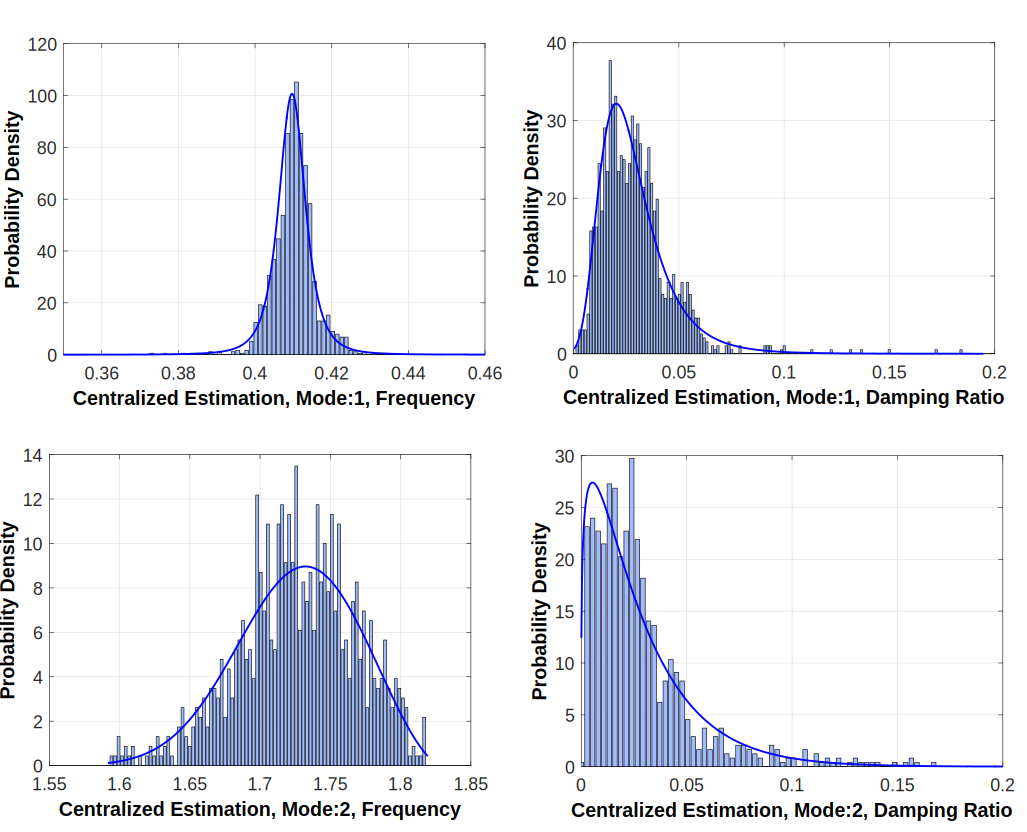
\includegraphics[trim=.5in .1in .5in .1in,width=2.8in]{Central_VM}
\caption{Estimates from centralized estimation with voltage magnitude signals; TOP: PDF of Mode 1 frequency (left), PDF of Mode 1 damping ratio (right); BOTTOM: PDF of Mode 2 frequency (left), PDF of Mode 2 damping ratio (right).}\label{centralVM}
\end{minipage}\qquad
\begin{minipage}[b]{.45\textwidth}
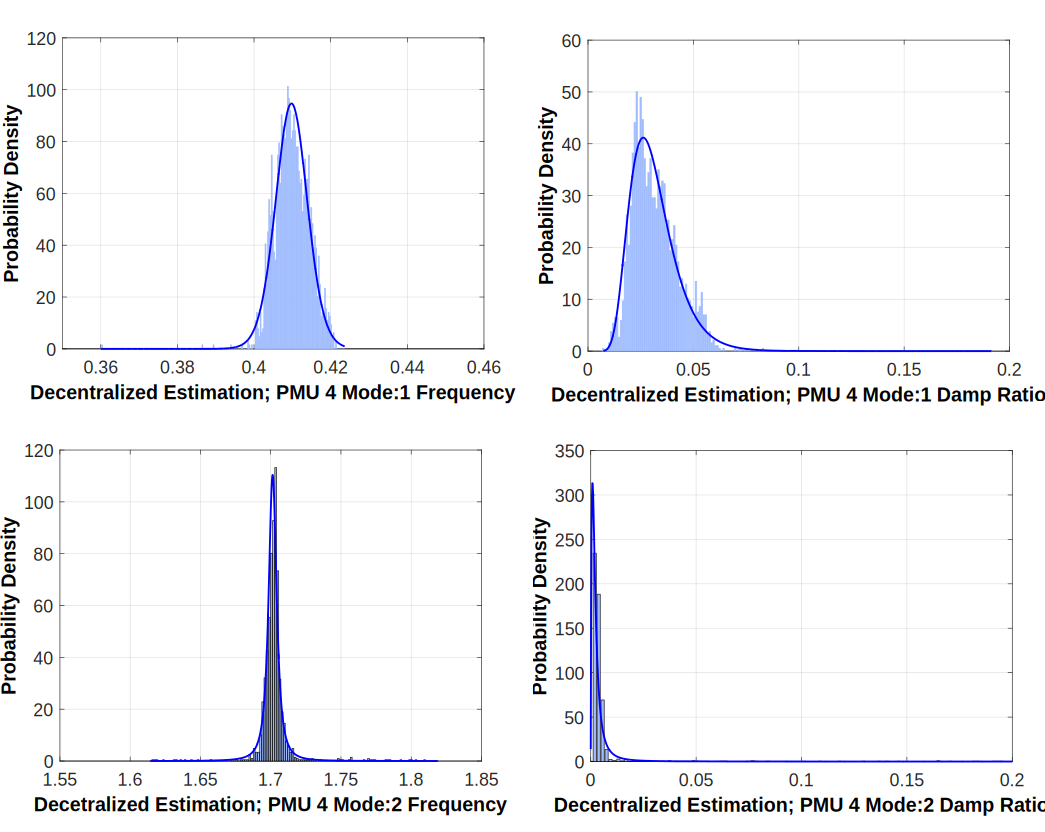
\includegraphics[trim=.1in .1in .1in .1in,width=3.05in]{Decentral_VM}
\caption{Estimates from decentralized estimation with voltage magnitude signals; TOP: PDF of Mode 1 frequency (left), PDF of Mode 1 damping ratio (right); BOTTOM: PDF of Mode 2 frequency (left), PDF of Mode 2 damping ratio (right).}\label{decentralVM}
\end{minipage}
\end{figure*}

\subsection{Voltage Magnitude Signals}
\vspace{-0.2em}
Positive sequence voltage phasor magnitudes acquired form the four PMUs were used as input signals for the mode-meter application. PDF plots of the estimates were obtained. Results from centralized estimation architecture show high density of estimates around mode 1 with mean frequency and standard deviation [0.4093, 0.0076] Hz. For mode 2, the mean frequency and standard deviation of estimates are [1.7256, 0.0425] Hz. The mean and standard deviation of the frequency and damping of the two modes identified are presented in Table \ref{tab:result_central}. The summary of results in terms of PDF plots for centralized architecture is presented in Fig. \ref{centralVM}.

The next case aims to demonstrate the decentralized mode estimator which attempts to improve the identification of the local forced oscillation (mode 2). All the PMU data streams were processed individually. Based on data from PMU 4 at node 799, mean frequency and standard deviation calculated are [0.0425, 0.045] Hz for mode 1 and [1.702, 0.013] Hz for mode 2.  Fig. \ref{decentralVM} presents the PDF plots based on the estimates obtained using PMU 4 data in decentralized architecture. The plots also suggest high density of estimates with mean frequency of 0.41 Hz  and also around the frequency of 1.7 Hz. The damping ratio of the forced oscillation is estimated to be 0.68\% with a standard deviation of 2.75\%. This means the damping ratio is nearly 0\% as expected. The mean and standard deviation of the frequency and damping of the two modes identified by decentralized estimates from all the PMUs are presented in Table \ref{tab:result_decentral}.
\begin{table}[!h]
\vspace{-1em}
\renewcommand{\arraystretch}{1.2}
\caption{Statistical analysis of centralized mode estimates}
\label{tab:result_central}
\noindent
\centering
    \begin{minipage}{\linewidth} %Use the minipage environment to footnote tables
    \renewcommand\footnoterule{\vspace*{-5pt}} %to remove the horizontal rule above the table footnote
    \begin{center}
        \begin{tabular}{c c c c c c c c c}
            \toprule
             \multicolumn{4}{c}{Mode 1 }& \multicolumn{4}{c}{Mode 2}\\
            \cline{1-8}
             \multicolumn{2}{c}{Freq. (Hz)}& \multicolumn{2}{c}{Damp. (\%)} & \multicolumn{2}{c}{Freq. (Hz)}& \multicolumn{2}{c}{Damp. (\%)}\\
            \cline{1-8}
             $\mu $ \footnote{$\mu $: mean}& $\sigma $ \footnote{$\sigma $: Standard deviation}  & $\mu $ & $\sigma $ & $\mu $ & $\sigma $ & $\mu $ & $\sigma $\\
            \midrule
              .4093  & .0076 & 2.84 & 1.7 & 1.726 & .0425 & 2.78 & 2.79\\
            
            \bottomrule
        \end{tabular}
        \end{center}
    \end{minipage}
\end{table}

\begin{table}[!b]
%% increase table row spacing, adjust to taste
\renewcommand{\arraystretch}{1.2}
%% if using array.sty, it might be a good idea to tweak the value of
%% \extrarowheight as needed to properly center the text within the cells
%
\caption{Statistical analysis of  decentralized mode estimates}
\label{tab:result_decentral}
\noindent
\centering
    \begin{minipage}{\linewidth} %Use the minipage environment to footnote tables
    \renewcommand\footnoterule{\vspace*{-5pt}} %to remove the horizontal rule above the table footnote
    \begin{center}
        \begin{tabular}{c c c c c c c c c c}
            \toprule
            \multirow{2}{*}{} & \multicolumn{4}{c}{Mode 1 }& \multicolumn{4}{c}{Mode 2}\\
            \cline{2-9}
            \multirow{2}{*}{PMU ID} & \multicolumn{2}{c}{Freq. (Hz)}& \multicolumn{2}{c}{Damp. (\%)} & \multicolumn{2}{c}{Freq. (Hz)}& \multicolumn{2}{c}{Damp. (\%)}\\
            \cline{2-9}
             & $\mu $ & $\sigma $  & $\mu $ & $\sigma $ & $\mu $ & $\sigma $ & $\mu $ & $\sigma $\\
            \midrule
            PMU 1 & .41  & .054 & 3.11 & 1.16 & 1.71 & .071 & 4.68 & 5.55\\
            PMU 2 & .41  & .049 & 3.15 & 1.12 & 1.71 & .047 & 3.11 & 5.04\\
            PMU 3 & .41  & .053 & 3.14 & 1.17 & 1.705 &.022 & 1.09 & 4.49\\
            PMU 4 & .41  & .045 & 3.13 & 1.09 & 1.702 & .013 & 0.68 & 4.41\\
            
            \bottomrule
        \end{tabular}
        \end{center}
    \end{minipage}
\end{table}


On comparison of mean and standard deviation of frequency and damping ratio estimates, it is evident that the local oscillation is better identified when using the decentralized architecture in case of voltage magnitude signals.    

\begin{comment}
\subsection{Voltage Angle Difference}
In this test, difference between voltage the angles measured at the four PMU nodes was used as input to the mode-meter application. The PDF plot based on centralized estimation is presented in Fig. \ref{central_VAD}. Similar plot for decentralized estimation using the data from PMU at node 799 is presented in Fig. \ref{decentral_VAD}.  

Both the PDF plots indicate the success of mode-meter application in estimating the inter-area oscillation at 0.42 HZ as well as the local forced oscillation at 1.7 Hz. 

\begin{figure*}[!ht]
\centering
\begin{minipage}[b]{.45\textwidth}
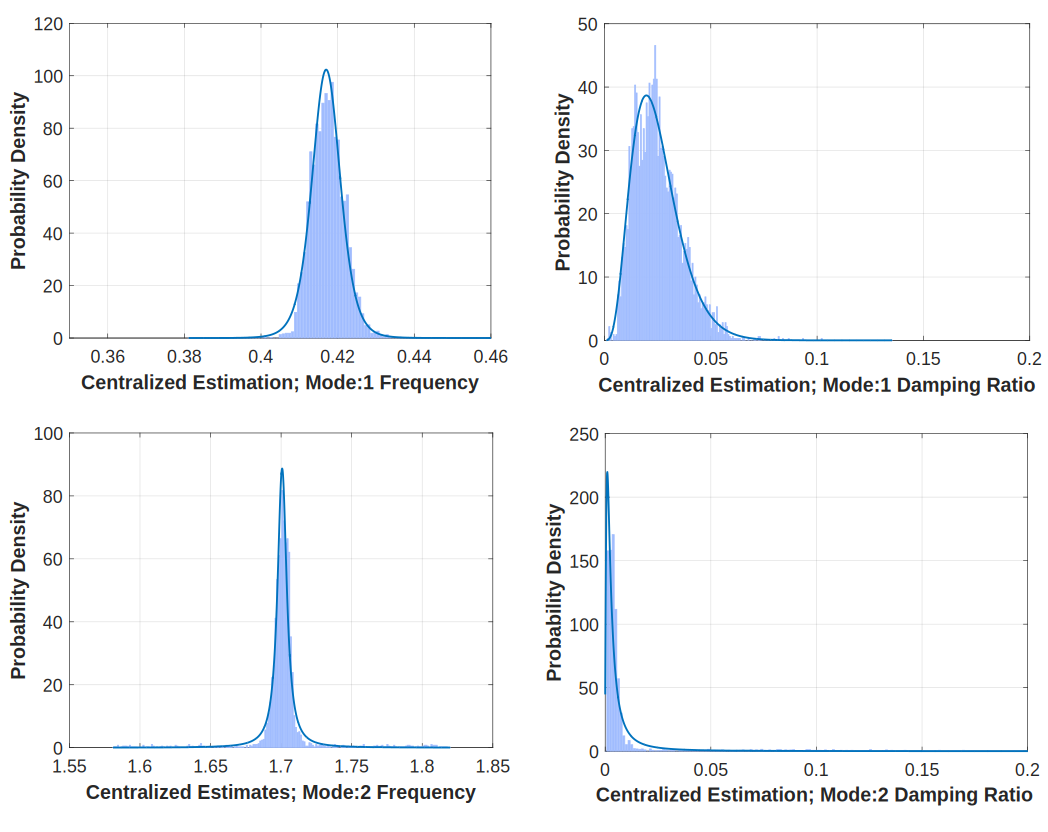
\includegraphics[trim=.4in .1in .5in .1in,width=2.8in]{Central_VAD}
\caption{Estimates from centralized estimation with difference in angles signals; TOP: PDF of Mode 1 frequency (left), PDF of Mode 1 damping ratio (right); BOTTOM: PDF of Mode 2 frequency (left), PDF of Mode 2 damping ratio (right).}\label{central_VAD}
\end{minipage}\qquad
\begin{minipage}[b]{.45\textwidth}
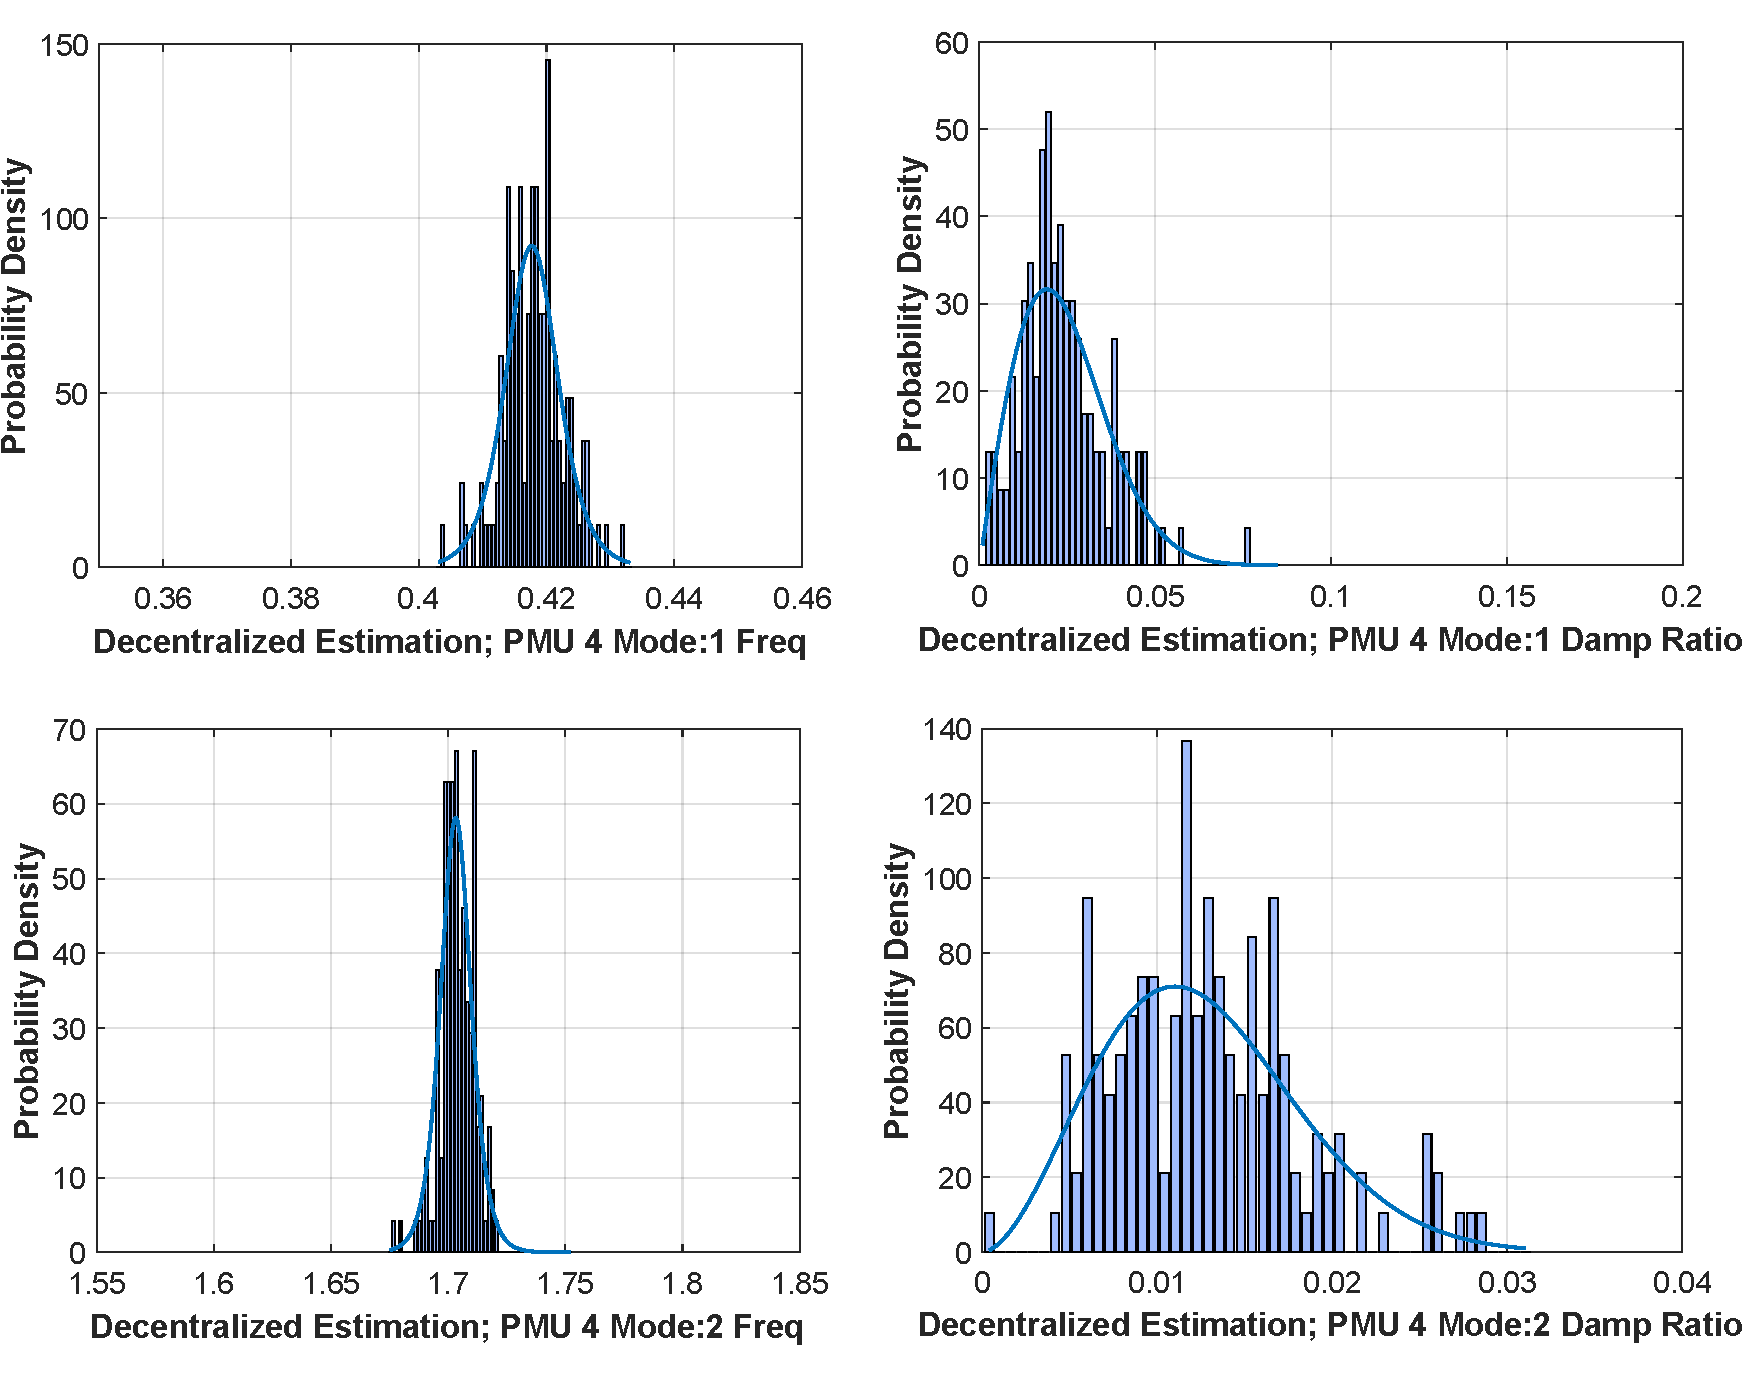
\includegraphics[trim=.1in .1in .1in .1in,width=3.05in]{Decentral_VAD}
\caption{Estimates from decentralized estimation with difference in angles signals; TOP: PDF of Mode 1 frequency (left), PDF of Mode 1 damping ratio (right); BOTTOM: PDF of Mode 2 frequency (left), PDF of Mode 2 damping ratio (right).}\label{decentral_VAD}
\end{minipage}
\end{figure*}
\end{comment}


\section{Conclusion} \label{conclusion}
A mode-meter application was tested and validated in a real-time experimental environment using PMU data streams. The application was run in two different architectures: centralized and decentralized. Voltage magnitude estimates from PMUs were tested as input signals to both architectures.  It was shown that the application was able to detect the major inter-area oscillations using both architectures.  It was found out that in case of voltage magnitude signals, the decentralized architecture provides better estimates for the localized oscillations. One more scenario, testing the mode-meter  application using measured voltage angle differences as input signals would be presented in the full paper. 

% use section* for acknowledgement


% can use a bibliography generated by BibTeX as a .bbl file
% BibTeX documentation can be easily obtained at:
% http://www.ctan.org/tex-archive/biblio/bibtex/contrib/doc/
% The IEEEtran BibTeX style support page is at:
% http://www.michaelshell.org/tex/ieeetran/bibtex/
%\bibliographystyle{IEEEtran}
% argument is your BibTeX string definitions and bibliography database(s)
%\bibliography{IEEEabrv,../bib/paper}
%
% <OR> manually copy in the resultant .bbl file
% set second argument of \begin to the number of references
% (used to reserve space for the reference number labels box)
\begin{thebibliography}{16}

\bibitem{gm2016}
R. S. Singh, H. Hooshyar and Luigi Vanfretti, ```In Silico' Testing of a Decentralized PMU
Data-Based Power Systems Mode Estimator," in \emph{Proc. 2016 IEEE Power and Energy Society General Meeting Conf.}, pp. 315-320. [Online]. Available KTH Diva Portal: \url{http://kth.diva-portal.org/smash/get/diva2:917903/FULLTEXT01.pdf}

\bibitem{hauer1}
J.F. Hauer, D.J.  Trudnowski, J.G. and DeSteese, ``A Perspective on WAMS Analysis Tools for Tracking of Oscillatory Dynamics," in \emph{Proc. IEEE Power Engineering Society General Meeting 2007}, June 2007, pp. 1-10.

\bibitem{mani2}
J. Ning, S.A.N. Samadi, V. Venkatasubramanian, ``Two-Level Ambient Oscillation Modal Estimation From Synchrophasor Measurements", in \emph{IEEE Trans. Power Systems}, vol. 30, No. 6, pp. 2913-2922, Aug. 2015.

\bibitem{taskforce}
\emph{Identification of Electromechanical Modes in Power Systems}, IEEE Task Force Report, Jun. 2012.

\bibitem{s3dk}
L. Vanfretti, V. H. Aarstrand, M. S. Almas, V. S. Perić and J. O. Gjerde, ``A software development toolkit for real-time synchrophasor applications" in \emph{Proc. PowerTech (POWERTECH), 2013 IEEE Grenoble, Grenoble}, 2013, pp. 1-6.

\bibitem{git}
Source code available at \url{https://github.com/SmarTS-Lab-Parapluie/S3DK}

\bibitem{refgrid}
H. Hooshyar, F. Mahmood, L. Vanfretti, M. Baudette, ``Specification,
implementation, and hardware-in-the-loop real-time simulation of an active distribution grid,” in \emph{Elsevier Sustainable Energy, Grids and Networks (SEGAN)}, Volume 3, September 2015, Pages 36-51.
\end{thebibliography}




% that's all folks
\end{document}


